\documentclass[11pt,a4paper]{article}

\usepackage{fontspec}
\setmainfont{Liberation Serif}
\setsansfont{Liberation Sans}
\setmonofont{Liberation Mono}

\usepackage[spanish,es-noshorthands]{babel}
\usepackage[margin=2.2cm,top=2.5cm,bottom=2.5cm,headheight=14pt]{geometry}
\usepackage{amsmath,amssymb}
\usepackage{booktabs}
\usepackage{longtable}
\usepackage{array}
\usepackage{colortbl}
\usepackage{fancyhdr}
\usepackage{tcolorbox}
\tcbuselibrary{breakable}
\usepackage{tikz}
\usetikzlibrary{shapes.geometric,arrows.meta,positioning,calc}
\usepackage{hyperref}

% Configuración de colores
\definecolor{sovietred}{RGB}{178,34,34}
\definecolor{techblue}{RGB}{24,76,120}
\definecolor{darkslate}{RGB}{44,62,80}
\definecolor{codebg}{RGB}{245,247,250}
\definecolor{tableheader}{RGB}{230,238,248}
\definecolor{rowalt}{RGB}{248,250,252}

\hypersetup{
    colorlinks=true,
    linkcolor=techblue,
    citecolor=sovietred,
    urlcolor=techblue,
    pdftitle={Elektronika MK-56: Referencia Técnica},
    pdfauthor={Ingeniería Retroinformática}
}

% Encabezados y pies de página
\pagestyle{fancy}
\fancyhf{}
\fancyhead[L]{\small\textcolor{darkslate}{\textbf{Elektronika MK-56} (\textit{Электроника МК-56})}}
\fancyhead[R]{\small\textcolor{darkslate}{Referencia Técnica y Microarquitectura}}
\fancyfoot[C]{\thepage}
\renewcommand{\headrulewidth}{0.4pt}
\renewcommand{\footrulewidth}{0pt}

% Estilo para cajas de notas y advertencias
\newtcolorbox{techbox}[2][]{
    colback=white,
    colframe=techblue,
    arc=1.5mm,
    fonttitle=\bfseries\sffamily,
    title=#2,
    coltitle=white,
    top=3mm,bottom=3mm,left=4mm,right=4mm,
    #1
}

\newtcolorbox{warnbox}[2][]{
    colback=white,
    colframe=sovietred,
    arc=1.5mm,
    fonttitle=\bfseries\sffamily,
    title=#2,
    coltitle=white,
    top=3mm,bottom=3mm,left=4mm,right=4mm,
    #1
}

\begin{document}

\begin{titlepage}
    \centering
    \vspace*{1.5cm}
    
    {\Huge\bfseries\textcolor{darkslate}{Elektronika MK-56}}\\[0.4cm]
    {\LARGE\textbf{\textit{Электроника МК-56}}}\\[1cm]
    
    {\Large\textcolor{techblue}{\textbf{Manual de Referencia Técnica y Microarquitectura}}}\\[0.3cm]
    {\large Especificación Formal de Hardware, Pila RPN, Opcodes y Control de Flujo}\\[1.5cm]
    
    \begin{tcolorbox}[colback=codebg,colframe=darkslate,width=0.85\textwidth,arc=2mm]
    \centering\small\sffamily
    \textbf{Documento Normativo para Desarrollo de Software Retroinformático:}\\
    Compiladores, Ensambladores, Desensambladores y Máquinas Virtuales
    \end{tcolorbox}
    
    \vspace{2cm}
    
    \begin{tabular}{ll}
        \textbf{Familia de Computación:} & URSS B3-34 / MK-54 / MK-56 / MK-61 \\
        \textbf{Arquitectura de CPU:}    & Serie K145 en tecnología PMOS \\
        \textbf{Modelo Operativo:}      & Notación Polaca Inversa (\textit{ПОЛИЗ}) \\
        \textbf{Capacidad de Memoria:}   & 98 pasos de programa, 14 registros de datos \\
        \textbf{Fecha de Publicación:}   & Octubre 2026 \\
    \end{tabular}

    \vfill
    {\small Documentación basada en el manual oficial técnico del fabricante de la URSS (\textit{Инструкция по эксплуатации})\\
    Traducción técnica, análisis de microarquitectura y diagramación en \LaTeX.}
\end{titlepage}

\tableofcontents
\newpage

\section{Arquitectura y Pila}

\subsection{Contexto Histórico y Circuitería Base}
La calculadora \textbf{Elektronika MK-56} (\textit{Электроника МК-56}) es la variante de sobremesa (alimentada por red eléctrica de $220\text{ V AC}, 50\text{ Hz}$) de la célebre familia de calculadoras microprogramables de segunda generación fabricadas en la Unión Soviética. Comparte microarquitectura, repertorio de instrucciones binarias y temporización con los modelos portátiles de bolsillo \textbf{Elektronika B3-34} (\textit{Электроника Б3-34}) y \textbf{Elektronika MK-54} (\textit{Электроника МК-54}).

El subsistema computacional está implementado mediante un conjunto de circuitos integrados LSI de alta densidad en tecnología PMOS pertenecientes a la \textbf{serie K145} (\textit{серия К145}):
\begin{itemize}
    \item \textbf{D4 (\textit{К145ИК1302} / K145IK1302):} Microprocesador principal de control, secuenciador y decodificador de teclado. Gestiona el ciclo de instrucción (fetch-decode-execute), el barrido del teclado, el refresco del tubo de visualización y el direccionamiento de la memoria de programa.
    \item \textbf{D5 (\textit{К145ИК1303} / K145IK1303):} Coprocesador aritmético y evaluador de funciones trascendentes. Implementa mediante microcódigo los algoritmos CORDIC y desarrollos en serie para trigonometría, logaritmos y funciones exponenciales.
    \item \textbf{D6 y D7 (\textit{К145ИР2} / K145IR2):} Registros dinámicos de desplazamiento / líneas de retardo de 1008 bits cada uno. Almacenan en serie los 14 registros de datos direccionables, los 4 niveles de la pila operativa y el registro de la pila de subrutinas.
    \item \textbf{D8 (\textit{К145АП1} / K145AP1):} Generador de reloj multifásico y generador de pulsos de sincronización para la lógica PMOS dinámica.
    \item \textbf{D1, D2, D3 (\textit{К161ПП1} / \textit{К161КН1} / Serie K161):} Llaves conmutadoras y excitadores de alta tensión para polarizar las rejillas y ánodos fosfóricos del tubo fluorescente.
\end{itemize}

\subsection{Formato de Números y Visualización (VFD)}
La salida de datos se efectúa a través de un tubo indicador fluorescente de vacío (\textit{VFD - вакуумно-люминесцентный индикатор}) de color verde esmeralda con 12 posiciones de dígitos físicos:
\begin{itemize}
    \item \textbf{Mantisa:} 8 dígitos decimales significativos más un dígito para el signo.
    \item \textbf{Exponente:} 2 dígitos decimales más un dígito para el signo del exponente.
    \item \textbf{Rango dinámico de representación numérica:}
    \[
    \pm 1 \cdot 10^{-99} \le |x| \le 9{,}9999999 \cdot 10^{99}
    \]
    \item \textbf{Conmutación entre Coma Fija y Coma Flotante:}
    \begin{itemize}
        \item Cuando el valor absoluto se halla comprendido en el intervalo $[10^{-7}, 10^8 - 1]$, la máquina lo visualiza en punto fijo natural con el separador decimal colocado en la columna correspondiente.
        \item Para magnitudes fuera de dicho rango, o de manera explícita tras pulsar la tecla \texttt{ВП} (\textit{Ввод Порядка} -- Entrada de Orden), el visualizador conmuta a notación científica:
        \[
        \pm M{,}MMMMMMM \quad \pm EE
        \]
    \end{itemize}
    \item \textbf{Condición de Error y Desbordamiento:} Cuando se produce una indeterminación matemática (división por cero, raíz de número negativo, logaritmo no positivo) o el exponente resultante excede $+99$, la máquina suspende la ejecución automática y muestra la palabra mnemónica \texttt{ЕГГОГ} (interpretación visual con dígitos de 7 segmentos del término anglosajón \textit{ERROR}).
\end{itemize}

\subsection{Arquitectura de la Pila RPN (\textit{ПОЛИЗ})}
La máquina procesa todas sus operaciones matemáticas mediante la Notación Polaca Inversa (en ruso: \textit{ПОЛИЗ -- Польская Инверсная Запись}). La pila de operandos está compuesta por \textbf{4 niveles activos} ($X, Y, Z, T$) y un \textbf{registro de respaldo} ($X_1$):

\begin{figure}[htbp]
    \centering
    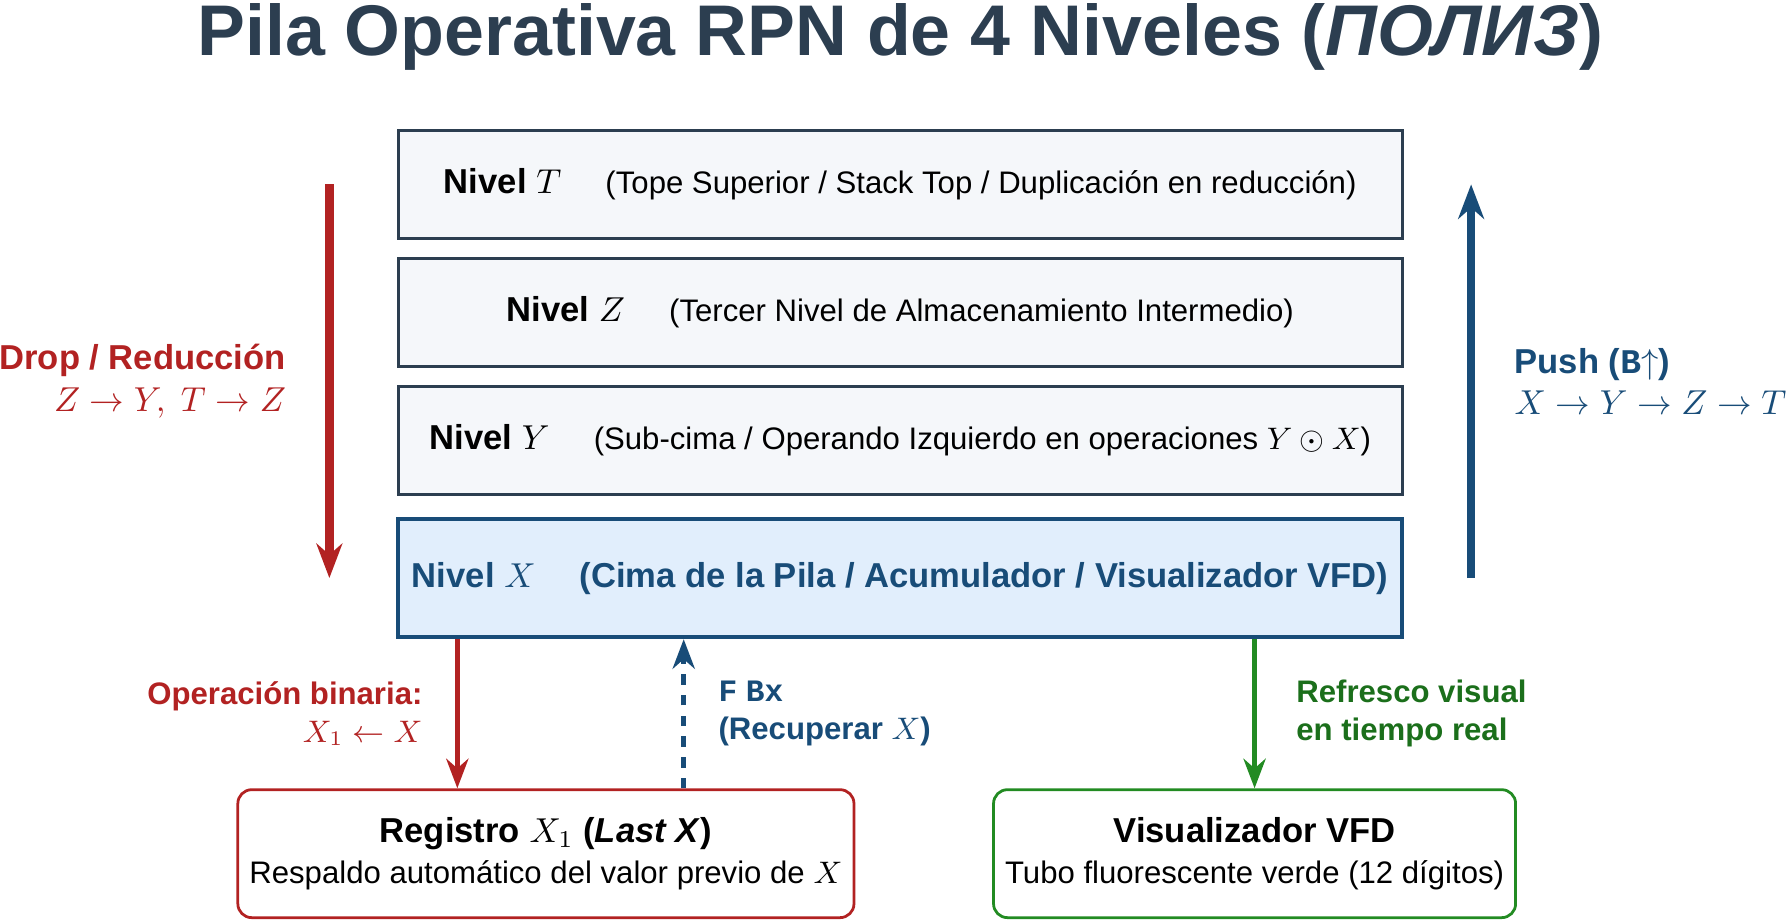
\includegraphics[width=0.92\textwidth]{figures/esquema_pila_es.png}
    \caption{Arquitectura de la Pila Operativa RPN (\textit{ПОЛИЗ}), registro de respaldo $X_1$ y visualizador VFD.}
    \label{fig:pila_es}
\end{figure}

\subsubsection{Definición de Registros}
\begin{enumerate}
    \item \textbf{Registro $X$ (\textit{Регистр X}):} Cima de la pila (\textit{Вершина стека}). Su valor es el único mostrado en pantalla. Ejerce el rol de acumulador por defecto para funciones unarias y destino de operaciones binarias.
    \item \textbf{Registro $Y$ (\textit{Регистр Y}):} Sub-cima. Constituye el primer operando (operando izquierdo) en operaciones diádicas: $Y \odot X$.
    \item \textbf{Registro $Z$ (\textit{Регистр Z}):} Almacenamiento intermedio de tercer nivel.
    \item \textbf{Registro $T$ (\textit{Регистр T}):} Nivel superior de la pila.
    \item \textbf{Registro $X_1$ (\textit{Регистр $X_1$ / Предыдущий результат}):} Registro desacoplado de copia sombra. Preserva automáticamente el contenido previo de $X$ antes de ejecutar cualquier operación aritmética binaria o función trascendente. Puede recuperarse en $X$ mediante \texttt{F} \texttt{Bx} (\textit{Восстановление X}).
\end{enumerate}

\subsection{Dinámica de Transición de Estados de la Pila}

\subsubsection{A. Introducción de Datos y Duplicación: \texorpdfstring{\texttt{В$\uparrow$}}{В-Enter} (\textit{Ввод в стек} / Enter)}
La pulsación de la tecla física \texttt{В$\uparrow$} empuja los niveles de la pila hacia arriba:
\[
\begin{pmatrix} X \\ Y \\ Z \\ T \end{pmatrix} \xrightarrow{\mathbf{B\uparrow}} \begin{pmatrix} X \\ X \\ Y \\ Z \end{pmatrix}
\]
El contenido de $X$ se copia íntegro en $Y$. El antiguo contenido de $T$ se descarta. El registro $X$ queda disponible para recibir los dígitos del siguiente operando sin perder el primer valor.

\subsubsection{B. Intercambio de la Cima y Sub-cima: \texorpdfstring{\texttt{$\leftrightarrow$}}{Swap} (\textit{Обмен X и Y} / Swap)}
Conmuta el valor de los registros $X$ e $Y$ sin alterar los niveles $Z$ y $T$:
\[
\begin{pmatrix} X \\ Y \\ Z \\ T \end{pmatrix} \xrightarrow{\mathbf{\leftrightarrow}} \begin{pmatrix} Y \\ X \\ Z \\ T \end{pmatrix}
\]

\subsubsection{C. Rotación Circular Descendente: \texorpdfstring{\texttt{F} $\circlearrowright$}{F Rotacion} (\textit{Кольцевое перемещение})}
Realiza un desplazamiento cíclico descendente de los cuatro registros de la pila:
\[
\begin{pmatrix} X \\ Y \\ Z \\ T \end{pmatrix} \xrightarrow{\mathbf{F\ \circlearrowright}} \begin{pmatrix} Y \\ Z \\ T \\ X \end{pmatrix}
\]
Cuatro rotaciones consecutivas (\texttt{F} $\circlearrowright$ $\times 4$) retornan la pila exactamente a su configuración inicial.

\subsubsection{D. Borrado del Acumulador: \texttt{Сх} (\textit{Сброс X} / Clear X)}
Pone a cero la cima de la pila sin perturbar el contenido ni la altura de los registros $Y$, $Z$ y $T$:
\[
\begin{pmatrix} X \\ Y \\ Z \\ T \end{pmatrix} \xrightarrow{\mathbf{Cx}} \begin{pmatrix} 0 \\ Y \\ Z \\ T \end{pmatrix}
\]

\subsubsection{E. Reducción en Operaciones Diádicas \texorpdfstring{($+$, $-$, $\times$, $\div$)}{(+, -, *, /)}}
En las operaciones aritméticas binarias ($Y \odot X$):
\begin{enumerate}
    \item El operando $X$ se almacena en el registro de respaldo $X_1$ ($X_1 \leftarrow X$).
    \item El resultado del cálculo se deposita en $X$ ($X \leftarrow Y \odot X$).
    \item El nivel $Z$ cae a $Y$ ($Y \leftarrow Z$).
    \item El nivel $T$ cae a $Z$ ($Z \leftarrow T$).
    \item El nivel $T$ \textbf{se preserva y duplica} ($T \leftarrow T$). Esta replicación de $T$ es una firma de diseño de los chips PMOS soviéticos.
\end{enumerate}
\[
\begin{pmatrix} X \\ Y \\ Z \\ T \end{pmatrix} \xrightarrow{\mathbf{+,\ -,\ \times,\ \div}} \begin{pmatrix} Y \odot X \\ Z \\ T \\ T \end{pmatrix}, \qquad X_1 \leftarrow X
\]

\subsubsection{F. Pila de Retorno de Subrutinas (\textit{Стек возврата})}
El procesador microprogramado K145IK1302 cuenta con una \textbf{pila hardware LIFO independiente de 5 niveles} dedicada a direcciones de retorno:
\begin{itemize}
    \item Cada instrucción \texttt{ПП} apila la dirección de retorno ($PC + 2$).
    \item Cada instrucción \texttt{В/О} desapila la dirección superior y ramifica hacia ella.
    \item \textbf{Límite de Anidamiento:} Si se efectúan más de 5 llamadas consecutivas sin retorno, se produce un desbordamiento circular perdiéndose la dirección más remota.
\end{itemize}

\newpage

\section{Mapa de Memoria y Registros}

\subsection{Memoria de Programa (\textit{ОЗУ команд})}
\begin{itemize}
    \item \textbf{Capacidad Total:} 98 pasos de programa.
    \item \textbf{Espacio de Direccionamiento:} Decimal lineal de dos dígitos: \texttt{00} a \texttt{97}.
    \item \textbf{Formato de Instrucción:} Tamaño de 1 byte por paso. Las operaciones con argumento de dirección ocupan dos pasos contiguos:
    \begin{itemize}
        \item Paso $N$: Opcode de salto o bifurcación (ej. \texttt{51} para \texttt{БП}).
        \item Paso $N+1$: Dirección numérica decimal de destino (ej. \texttt{25}).
    \end{itemize}
\end{itemize}

\subsubsection{Modos Operativos de la Máquina}
\begin{enumerate}
    \item \textbf{Modo Automático / Ejecución (\textit{АВТ} / \texttt{F ABT} o interruptor \textit{Р}):}
    Modo en el que el secuenciador ejecuta el código almacenado secuencialmente al pulsar \texttt{С/П} (\textit{Старт/Пуск}).
    \item \textbf{Modo Programación (\textit{ПРГ} / \texttt{F ПРГ} o interruptor \textit{ПРГ}):}
    Modo de edición directa de la memoria RAM. El visualizador VFD muestra el formato:
    \[
    \mathbf{AA \quad CC}
    \]
    Donde $\mathbf{AA}$ representa la dirección de memoria activa (\texttt{00} a \texttt{97}) y $\mathbf{CC}$ el código de operación almacenado. Las teclas \texttt{ШГ $\rightarrow$} y \texttt{ШГ $\leftarrow$} permiten desplazarse hacia adelante o hacia atrás en el programa paso a paso.
\end{enumerate}

\subsection{Registros de Datos Direccionables (\textit{Адресуемые регистры})}
La máquina provee \textbf{14 registros de memoria en RAM dinámica}, identificados unívocamente:
\[
RG0, RG1, RG2, RG3, RG4, RG5, RG6, RG7, RG8, RG9, RGa, RGb, RGc, RGd
\]
Cada registro contiene un número completo en coma flotante (8 dígitos de mantisa y 2 de exponente con signos respectivos).

\begin{center}
\small
\begin{tabular}{ccp{7.2cm}p{4.6cm}}
\toprule
\textbf{Registro} & \textbf{Tecla} & \textbf{Comportamiento en Modo Indirecto (\texttt{K})} & \textbf{Uso Común} \\
\midrule
$RG0$ & \texttt{0}       & Autodecremento en 1 ($RG0 \leftarrow RG0 - 1$) & Contador bucle / Puntero desc. \\
$RG1$ & \texttt{1}       & Autodecremento en 1 ($RG1 \leftarrow RG1 - 1$) & Contador bucle / Puntero desc. \\
$RG2$ & \texttt{2}       & Autodecremento en 1 ($RG2 \leftarrow RG2 - 1$) & Contador bucle / Puntero desc. \\
$RG3$ & \texttt{3}       & Autodecremento en 1 ($RG3 \leftarrow RG3 - 1$) & Contador bucle / Puntero desc. \\
\midrule
$RG4$ & \texttt{4}       & Autoincremento en 1 ($RG4 \leftarrow RG4 + 1$) & Puntero de memoria asc. \\
$RG5$ & \texttt{5}       & Autoincremento en 1 ($RG5 \leftarrow RG5 + 1$) & Puntero de memoria asc. \\
$RG6$ & \texttt{6}       & Autoincremento en 1 ($RG6 \leftarrow RG6 + 1$) & Puntero de memoria asc. \\
\midrule
$RG7$ & \texttt{7}       & Sin modificación automática ($RG7 \leftarrow RG7$) & Registro general de datos \\
$RG8$ & \texttt{8}       & Sin modificación automática ($RG8 \leftarrow RG8$) & Registro general de datos \\
$RG9$ & \texttt{9}       & Sin modificación automática ($RG9 \leftarrow RG9$) & Registro general de datos \\
$RGa$ & \texttt{.} ($a$) & Sin modificación automática ($RGa \leftarrow RGa$) & Registro general de datos \\
$RGb$ & \texttt{/-/} ($b$)& Sin modificación automática ($RGb \leftarrow RGb$) & Registro general de datos \\
$RGc$ & \texttt{ВП} ($c$)& Sin modificación automática ($RGc \leftarrow RGc$) & Registro general de datos \\
$RGd$ & \texttt{Сх} ($d$)& Sin modificación automática ($RGd \leftarrow RGd$) & Registro general de datos \\
\bottomrule
\end{tabular}
\end{center}

\subsection{Modos de Direccionamiento de Memoria}
\begin{enumerate}
    \item \textbf{Direccionamiento Directo:}
    \begin{itemize}
        \item \textbf{Almacenar:} \texttt{x$\to$П} $[R]$ (\textit{Запись X в регистр}). Copia el valor del acumulador $X$ en el registro $R$ ($0 \le R \le d$). El contenido de $X$ permanece inalterado.
        \item \textbf{Recuperar:} \texttt{П$\to$x} $[R]$ (\textit{Вызов из регистра в X}). Copia el contenido del registro $R$ en $X$, empujando previamente la pila hacia arriba.
    \end{itemize}
    \item \textbf{Direccionamiento Indirecto (Prefijo \texttt{K}):}
    \begin{itemize}
        \item \textbf{Escritura Indirecta:} \texttt{K} \texttt{x$\to$П} $[R]$. Utiliza la parte entera de $R$ como dirección del registro destino final.
        \item \textbf{Lectura Indirecta:} \texttt{K} \texttt{П$\to$x} $[R]$. Utiliza la parte entera de $R$ como dirección del registro origen y copia su contenido a $X$.
    \end{itemize}
\end{enumerate}

\begin{techbox}{Regla Crítica de Modificación Automática en Acceso Indirecto}
Antes de ejecutar la transferencia física o el salto indirecto con el prefijo \texttt{K}:
\begin{itemize}
    \item Si $R \in \{0, 1, 2, 3\}$: Se resta $1$ al registro puntero ($R \leftarrow R - 1$).
    \item Si $R \in \{4, 5, 6\}$: Se suma $1$ al registro puntero ($R \leftarrow R + 1$).
    \item Si $R \in \{7, 8, 9, a, b, c, d\}$: El valor de $R$ no se altera.
\end{itemize}
\end{techbox}

\newpage

\section{Repertorio de Instrucciones (Opcodes)}

La siguiente relación compila la totalidad del catálogo de instrucciones de la Elektronika MK-56 según la especificación técnica oficial del fabricante (\textbf{Tabla 4 del manual de fábrica}).

\subsection{Convención de Mapeo Hexadecimal en el Tubo VFD}
Los circuitos integrados K145IK1302 representan los nibbles hexadecimales en el visualizador de 7 segmentos de acuerdo con el estándar soviético:
\begin{center}
\begin{tabular}{ccp{8cm}}
\toprule
\textbf{Nibble Hex} & \textbf{Glifo en VFD} & \textbf{Significado / Segmentos Iluminados} \\
\midrule
\texttt{0x0} -- \texttt{0x9} & \texttt{0} -- \texttt{9} & Dígitos decimales estándar \\
\texttt{0xA} (10) & \texttt{-} & Segmento central horizontal (gión) \\
\texttt{0xB} (11) & \texttt{L} & Segmentos vertical inferior e inferior horizontal (L mayúscula) \\
\texttt{0xC} (12) & \texttt{C} & Segmentos superior, vertical superior/inferior e inferior (C mayúscula) \\
\texttt{0xD} (13) & \texttt{Г} & Letra cirílica Gamma (segmento superior y vertical izquierdo) \\
\texttt{0xE} (14) & \texttt{E} & Letra E mayúscula \\
\texttt{0xF} (15) & \textit{blanco} & Dígito completamente apagado \\
\bottomrule
\end{tabular}
\end{center}

\begin{figure}[htbp]
    \centering
    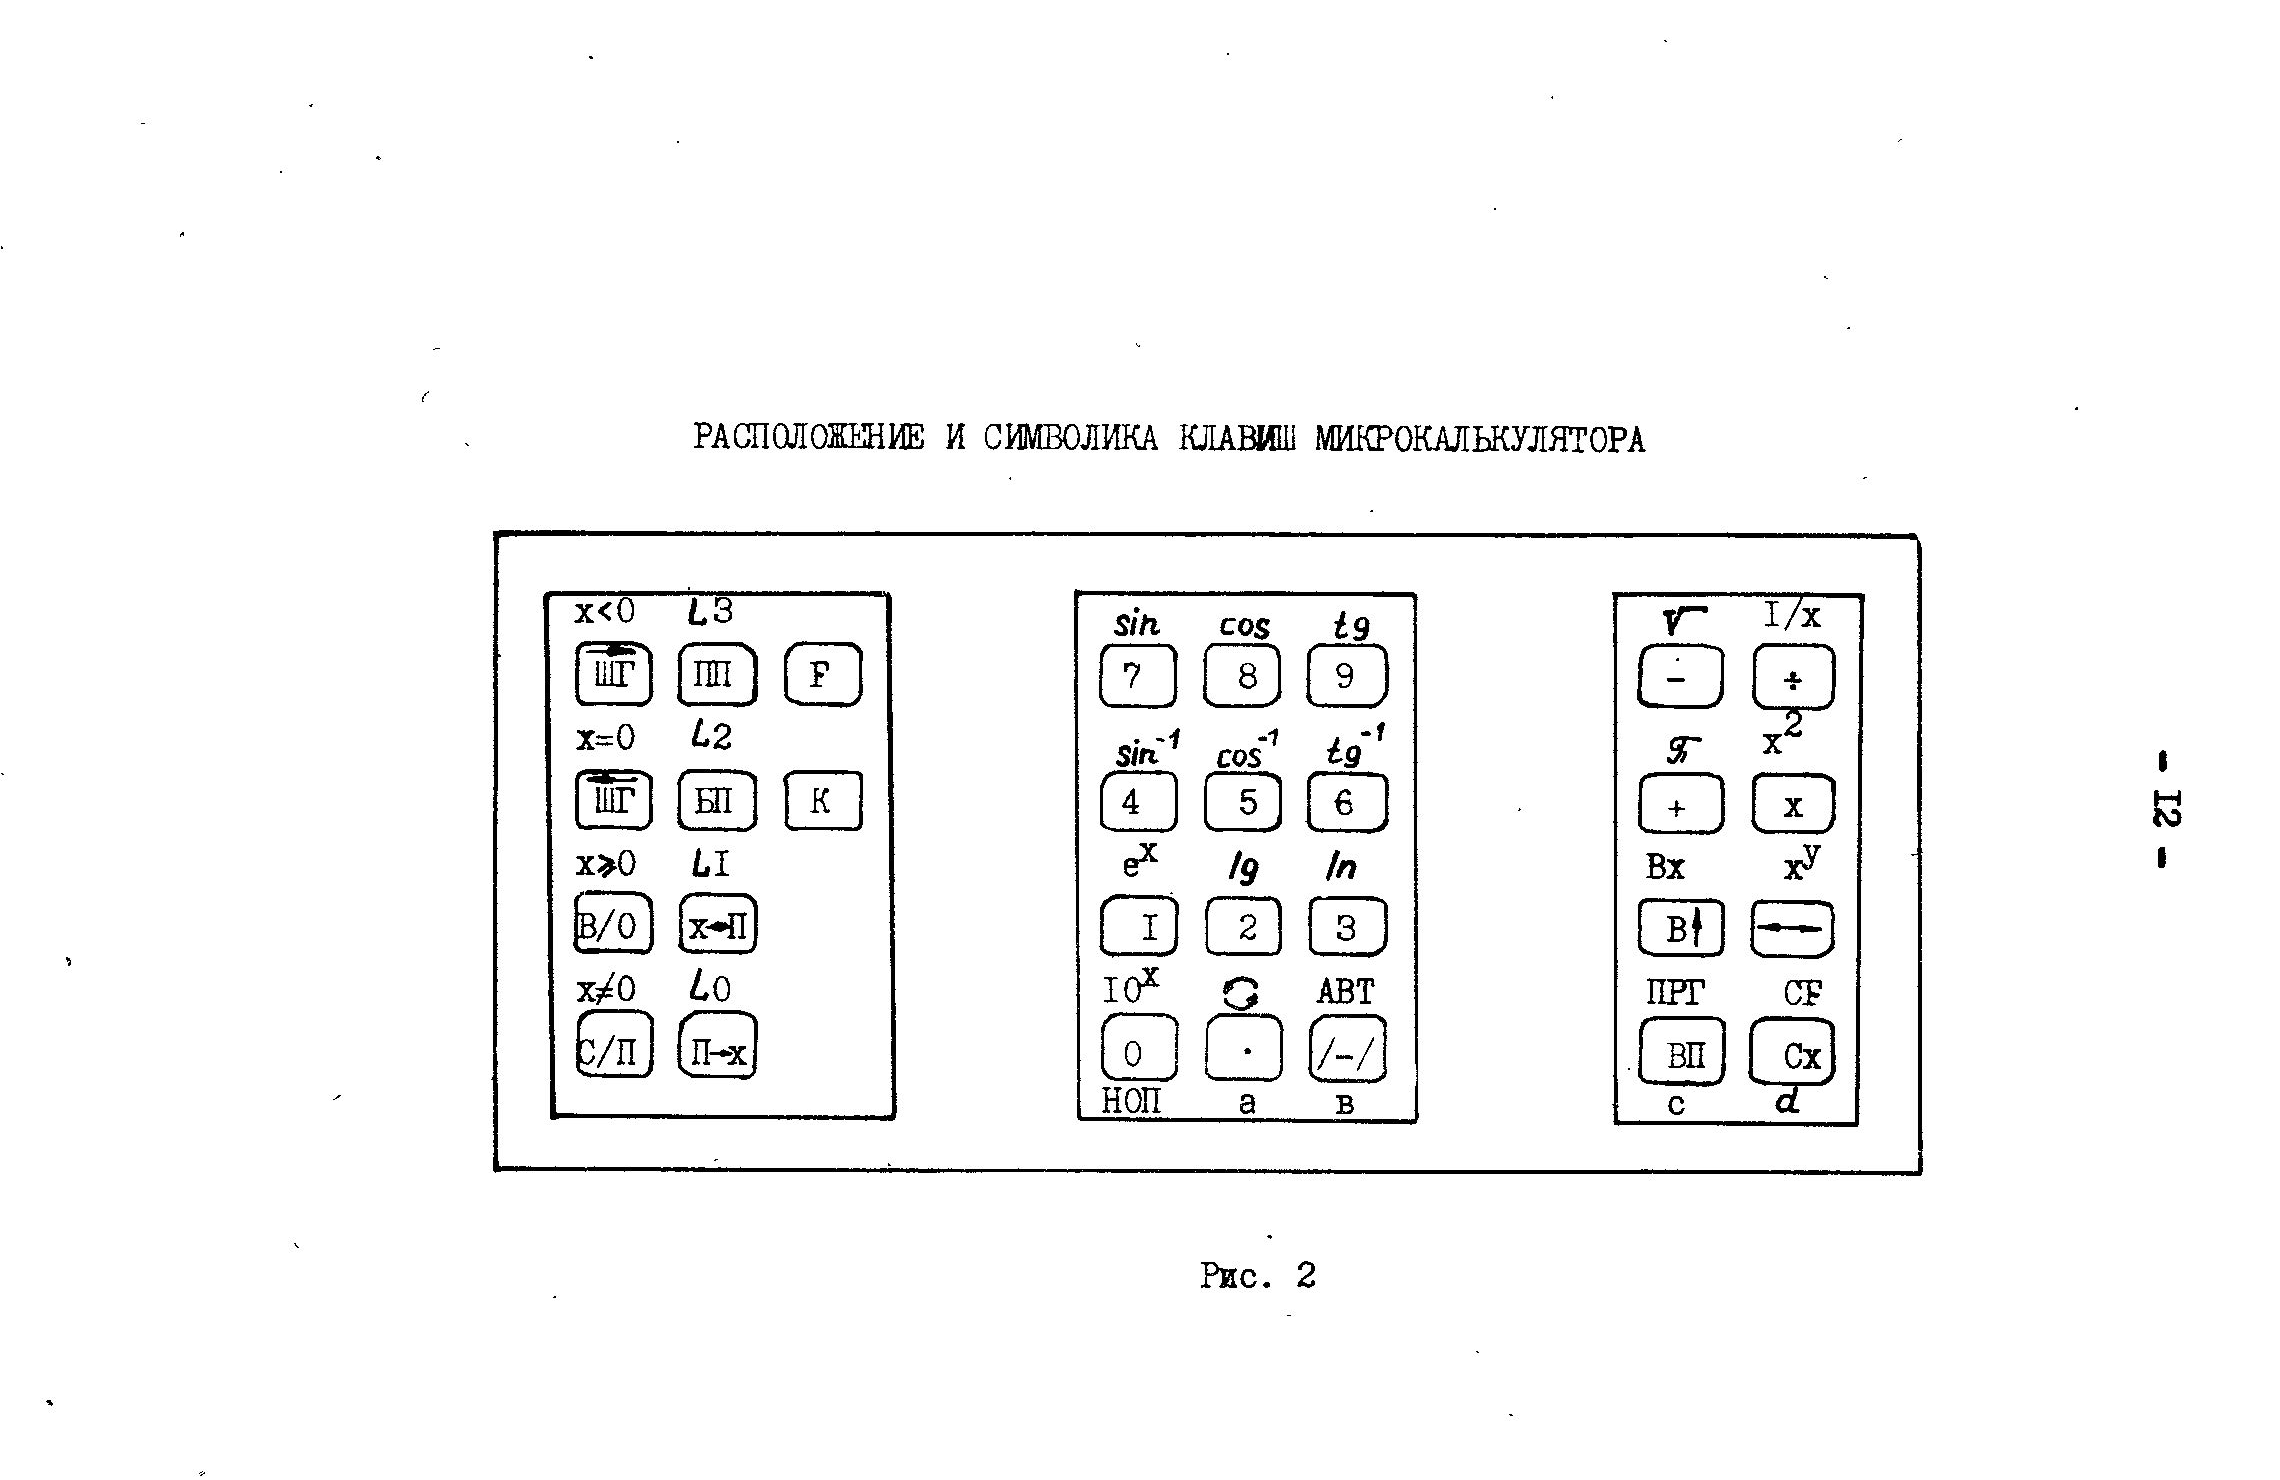
\includegraphics[width=0.90\textwidth]{figures/fig2_teclado_mk56.png}
    \caption{Disposición física y simbología de las teclas de la Elektronika MK-56 (Figura 2 del manual técnico oficial de fábrica).}
    \label{fig:teclado_mk56}
\end{figure}

\subsection{Tabla Oficial de Opcodes (Таблица 4)}

{\small
\setlength{\tabcolsep}{4pt}
\begin{longtable}{p{2.2cm}p{3.0cm}>{\centering\arraybackslash}p{1.0cm}>{\centering\arraybackslash}p{1.2cm}p{7.3cm}}
\toprule
\textbf{Tecla (Cirílico)} & \textbf{Nombre en Español} & \textbf{VFD} & \textbf{Hex} & \textbf{Semántica Formal y Efecto en la Pila} \\
\midrule
\endfirsthead
\toprule
\textbf{Tecla (Cirílico)} & \textbf{Nombre en Español} & \textbf{VFD} & \textbf{Hex} & \textbf{Semántica Formal y Efecto en la Pila} \\
\midrule
\endhead
\bottomrule
\endfoot
\texttt{0} & Cero & \texttt{00} & \texttt{0x00} & Carga el dígito literal 0 en el acumulador $X$ \\
\texttt{1} & Uno & \texttt{01} & \texttt{0x01} & Carga el dígito literal 1 en el acumulador $X$ \\
\texttt{2} & Dos & \texttt{02} & \texttt{0x02} & Carga el dígito literal 2 en el acumulador $X$ \\
\texttt{3} & Tres & \texttt{03} & \texttt{0x03} & Carga el dígito literal 3 en el acumulador $X$ \\
\texttt{4} & Cuatro & \texttt{04} & \texttt{0x04} & Carga el dígito literal 4 en el acumulador $X$ \\
\texttt{5} & Cinco & \texttt{05} & \texttt{0x05} & Carga el dígito literal 5 en el acumulador $X$ \\
\texttt{6} & Seis & \texttt{06} & \texttt{0x06} & Carga el dígito literal 6 en el acumulador $X$ \\
\texttt{7} & Siete & \texttt{07} & \texttt{0x07} & Carga el dígito literal 7 en el acumulador $X$ \\
\texttt{8} & Ocho & \texttt{08} & \texttt{0x08} & Carga el dígito literal 8 en el acumulador $X$ \\
\texttt{9} & Nueve & \texttt{09} & \texttt{0x09} & Carga el dígito literal 9 en el acumulador $X$ \\
\texttt{.} & Punto decimal & \texttt{0-} & \texttt{0x0A} & Fija el punto decimal de la mantisa activa \\
\texttt{/-/} & Cambio de signo & \texttt{0L} & \texttt{0x0B} & Invierte el signo del acumulador: $X \leftarrow -X$ \\
\texttt{ВП} & Entrada de orden & \texttt{0C} & \texttt{0x0C} & Conmuta al modo de introducción del exponente \\
\texttt{Сх} & Borrar X & \texttt{0Г} & \texttt{0x0D} & Limpia el acumulador: $X \leftarrow 0$; pila inalterada \\
\texttt{В$\uparrow$} & Enter / Pila & \texttt{0E} & \texttt{0x0E} & Empuja pila: $X \to Y, Y \to Z, Z \to T$; conserva $X$ \\
\midrule
\texttt{+} & Suma & \texttt{10} & \texttt{0x10} & $X \leftarrow Y + X;\; Z \to Y;\; T \to Z;\; X_1 \leftarrow X$ \\
\texttt{-} & Resta & \texttt{11} & \texttt{0x11} & $X \leftarrow Y - X;\; Z \to Y;\; T \to Z;\; X_1 \leftarrow X$ \\
\texttt{$\times$} & Multiplicación & \texttt{12} & \texttt{0x12} & $X \leftarrow Y \times X;\; Z \to Y;\; T \to Z;\; X_1 \leftarrow X$ \\
\texttt{$\div$} & División & \texttt{13} & \texttt{0x13} & $X \leftarrow Y / X;\; Z \to Y;\; T \to Z;\; X_1 \leftarrow X$ ($X \ne 0$) \\
\texttt{$\leftrightarrow$} & Intercambio X-Y & \texttt{14} & \texttt{0x14} & Swap: $X \leftrightarrow Y$; registros $Z$ y $T$ inalterados \\
\texttt{F 10\textasciicircum x} & Potencia de 10 & \texttt{15} & \texttt{0x15} & $X \leftarrow 10^X;\; X_1 \leftarrow X$ \\
\texttt{F e\textasciicircum x} & Exponencial & \texttt{16} & \texttt{0x16} & $X \leftarrow e^X;\; X_1 \leftarrow X$ \\
\texttt{F lg} & Logaritmo base 10 & \texttt{17} & \texttt{0x17} & $X \leftarrow \log_{10}(X);\; X_1 \leftarrow X$ ($X > 0$) \\
\texttt{F ln} & Logaritmo natural & \texttt{18} & \texttt{0x18} & $X \leftarrow \ln(X);\; X_1 \leftarrow X$ ($X > 0$) \\
\texttt{F arcsin} & Arco seno & \texttt{19} & \texttt{0x19} & $X \leftarrow \arcsin(X);\; X_1 \leftarrow X$ ($|X| \le 1$) \\
\texttt{F arccos} & Arco coseno & \texttt{1-} & \texttt{0x1A} & $X \leftarrow \arccos(X);\; X_1 \leftarrow X$ ($|X| \le 1$) \\
\texttt{F arctg} & Arco tangente & \texttt{1L} & \texttt{0x1B} & $X \leftarrow \arctan(X);\; X_1 \leftarrow X$ \\
\texttt{F sin} & Seno & \texttt{1C} & \texttt{0x1C} & $X \leftarrow \sin(X)$; unidad según conmutador angular \\
\texttt{F cos} & Coseno & \texttt{1Г} & \texttt{0x1D} & $X \leftarrow \cos(X)$; unidad según conmutador angular \\
\texttt{F tg} & Tangente & \texttt{1E} & \texttt{0x1E} & $X \leftarrow \tan(X)$; unidad según conmutador angular \\
\midrule
\texttt{F $\pi$} & Constante Pi & \texttt{20} & \texttt{0x20} & Carga $\pi \approx 3{,}1415926$ en $X$; empuja la pila \\
\texttt{F $\sqrt{x}$} & Raíz cuadrada & \texttt{21} & \texttt{0x21} & $X \leftarrow \sqrt{X};\; X_1 \leftarrow X$ ($X \ge 0$) \\
\texttt{F x\textasciicircum 2} & Cuadrado & \texttt{22} & \texttt{0x22} & $X \leftarrow X^2;\; X_1 \leftarrow X$ \\
\texttt{F 1/x} & Inverso & \texttt{23} & \texttt{0x23} & $X \leftarrow 1/X;\; X_1 \leftarrow X$ ($X \ne 0$) \\
\texttt{F x\textasciicircum y} & Potencia arbitraria & \texttt{24} & \texttt{0x24} & $X \leftarrow Y^X;\; Z \to Y;\; T \to Z;\; X_1 \leftarrow X$ \\
\midrule
\texttt{x$\to$П 0} & Guardar en RG0 & \texttt{40} & \texttt{0x40} & $RG0 \leftarrow X$; acumulador $X$ inalterado \\
\texttt{x$\to$П 1} & Guardar en RG1 & \texttt{41} & \texttt{0x41} & $RG1 \leftarrow X$; acumulador $X$ inalterado \\
\texttt{x$\to$П 2} & Guardar en RG2 & \texttt{42} & \texttt{0x42} & $RG2 \leftarrow X$; acumulador $X$ inalterado \\
\texttt{x$\to$П 3} & Guardar en RG3 & \texttt{43} & \texttt{0x43} & $RG3 \leftarrow X$; acumulador $X$ inalterado \\
\texttt{x$\to$П 4} & Guardar en RG4 & \texttt{44} & \texttt{0x44} & $RG4 \leftarrow X$; acumulador $X$ inalterado \\
\texttt{x$\to$П 5} & Guardar en RG5 & \texttt{45} & \texttt{0x45} & $RG5 \leftarrow X$; acumulador $X$ inalterado \\
\texttt{x$\to$П 6} & Guardar en RG6 & \texttt{46} & \texttt{0x46} & $RG6 \leftarrow X$; acumulador $X$ inalterado \\
\texttt{x$\to$П 7} & Guardar en RG7 & \texttt{47} & \texttt{0x47} & $RG7 \leftarrow X$; acumulador $X$ inalterado \\
\texttt{x$\to$П 8} & Guardar en RG8 & \texttt{48} & \texttt{0x48} & $RG8 \leftarrow X$; acumulador $X$ inalterado \\
\texttt{x$\to$П 9} & Guardar en RG9 & \texttt{49} & \texttt{0x49} & $RG9 \leftarrow X$; acumulador $X$ inalterado \\
\texttt{x$\to$П a} & Guardar en RGa & \texttt{4-} & \texttt{0x4A} & $RGa \leftarrow X$; acumulador $X$ inalterado \\
\texttt{x$\to$П b} & Guardar en RGb & \texttt{4L} & \texttt{0x4B} & $RGb \leftarrow X$; acumulador $X$ inalterado \\
\texttt{x$\to$П c} & Guardar en RGc & \texttt{4C} & \texttt{0x4C} & $RGc \leftarrow X$; acumulador $X$ inalterado \\
\texttt{x$\to$П d} & Guardar en RGd & \texttt{4Г} & \texttt{0x4D} & $RGd \leftarrow X$; acumulador $X$ inalterado \\
\midrule
\texttt{С/П} & Start / Stop & \texttt{50} & \texttt{0x50} & Detiene o reanuda la ejecución en modo automático \\
\texttt{БП} & Salto incondicional & \texttt{51} & \texttt{0x51} & Bifurcación absoluta: $PC \leftarrow \text{byte inmediato } (N+1)$ \\
\texttt{В/О} & Retorno / Origen & \texttt{52} & \texttt{0x52} & Retorno subrutina ($PC \leftarrow \text{pop}$) o resetea a \texttt{00} \\
\texttt{ПП} & Llamada subrutina & \texttt{53} & \texttt{0x53} & Apila $PC+2$ en stack retorno; $PC \leftarrow \text{byte } (N+1)$ \\
\texttt{K НОП} & No Operación & \texttt{54} & \texttt{0x54} & NOP: No ejecuta cambios; avanza a $PC+1$ \\
\texttt{F x$\ne$0} & Salto si $X \ne 0$ & \texttt{57} & \texttt{0x57} & \textbf{Invertido:} Si $X = 0 \Rightarrow$ salta a $N+1$; Si $X \ne 0 \Rightarrow PC+2$ \\
\texttt{F L2} & Bucle contador RG2 & \texttt{58} & \texttt{0x58} & $RG2 \leftarrow RG2-1$; Si $RG2 \ne 0 \Rightarrow$ salta; Si 0 $\Rightarrow PC+2$ \\
\texttt{F x$\ge$0} & Salto si $X \ge 0$ & \texttt{59} & \texttt{0x59} & \textbf{Invertido:} Si $X < 0 \Rightarrow$ salta a $N+1$; Si $X \ge 0 \Rightarrow PC+2$ \\
\texttt{F L3} & Bucle contador RG3 & \texttt{5-} & \texttt{0x5A} & $RG3 \leftarrow RG3-1$; Si $RG3 \ne 0 \Rightarrow$ salta; Si 0 $\Rightarrow PC+2$ \\
\texttt{F L1} & Bucle contador RG1 & \texttt{5L} & \texttt{0x5B} & $RG1 \leftarrow RG1-1$; Si $RG1 \ne 0 \Rightarrow$ salta; Si 0 $\Rightarrow PC+2$ \\
\texttt{F x$<$0} & Salto si $X < 0$ & \texttt{5C} & \texttt{0x5C} & \textbf{Invertido:} Si $X \ge 0 \Rightarrow$ salta a $N+1$; Si $X < 0 \Rightarrow PC+2$ \\
\texttt{F L0} & Bucle contador RG0 & \texttt{5Г} & \texttt{0x5D} & $RG0 \leftarrow RG0-1$; Si $RG0 \ne 0 \Rightarrow$ salta; Si 0 $\Rightarrow PC+2$ \\
\texttt{F x$=$0} & Salto si $X = 0$ & \texttt{5E} & \texttt{0x5E} & \textbf{Invertido:} Si $X \ne 0 \Rightarrow$ salta a $N+1$; Si $X = 0 \Rightarrow PC+2$ \\
\midrule
\texttt{П$\to$x 0} & Leer de RG0 & \texttt{60} & \texttt{0x60} & Carga $RG0$ en $X$; empuja previamente la pila \\
\texttt{П$\to$x 1} & Leer de RG1 & \texttt{61} & \texttt{0x61} & Carga $RG1$ en $X$; empuja previamente la pila \\
\texttt{П$\to$x 2} & Leer de RG2 & \texttt{62} & \texttt{0x62} & Carga $RG2$ en $X$; empuja previamente la pila \\
\texttt{П$\to$x 3} & Leer de RG3 & \texttt{63} & \texttt{0x63} & Carga $RG3$ en $X$; empuja previamente la pila \\
\texttt{П$\to$x 4} & Leer de RG4 & \texttt{64} & \texttt{0x64} & Carga $RG4$ en $X$; empuja previamente la pila \\
\texttt{П$\to$x 5} & Leer de RG5 & \texttt{65} & \texttt{0x65} & Carga $RG5$ en $X$; empuja previamente la pila \\
\texttt{П$\to$x 6} & Leer de RG6 & \texttt{66} & \texttt{0x66} & Carga $RG6$ en $X$; empuja previamente la pila \\
\texttt{П$\to$x 7} & Leer de RG7 & \texttt{67} & \texttt{0x67} & Carga $RG7$ en $X$; empuja previamente la pila \\
\texttt{П$\to$x 8} & Leer de RG8 & \texttt{68} & \texttt{0x68} & Carga $RG8$ en $X$; empuja previamente la pila \\
\texttt{П$\to$x 9} & Leer de RG9 & \texttt{69} & \texttt{0x69} & Carga $RG9$ en $X$; empuja previamente la pila \\
\texttt{П$\to$x a} & Leer de RGa & \texttt{6-} & \texttt{0x6A} & Carga $RGa$ en $X$; empuja previamente la pila \\
\texttt{П$\to$x b} & Leer de RGb & \texttt{6L} & \texttt{0x6B} & Carga $RGb$ en $X$; empuja previamente la pila \\
\texttt{П$\to$x c} & Leer de RGc & \texttt{6C} & \texttt{0x6C} & Carga $RGc$ en $X$; empuja previamente la pila \\
\texttt{П$\to$x d} & Leer de RGd & \texttt{6Г} & \texttt{0x6D} & Carga $RGd$ en $X$; empuja previamente la pila \\
\midrule
\texttt{K x$\ne$0 [R]} & Salto cond. ind. & \texttt{70}--\texttt{7Г} & \texttt{0x70}--\texttt{0x7D} & Test indirecto $X \ne 0$ vía $RG0..RGd$ \\
\texttt{K БП [R]} & Salto incond. ind. & \texttt{80}--\texttt{8Г} & \texttt{0x80}--\texttt{0x8D} & Salto indirecto incondicional a dir. en $R$ \\
\texttt{K x$\ge$0 [R]} & Salto cond. ind. & \texttt{90}--\texttt{9Г} & \texttt{0x90}--\texttt{0x9D} & Test indirecto $X \ge 0$ vía $RG0..RGd$ \\
\texttt{K ПП [R]} & Subrutina ind. & \texttt{-0}--\texttt{-Г} & \texttt{0xA0}--\texttt{0xAD} & Llamada indirecta a subrutina vía $RG0..RGd$ \\
\texttt{K x$\to$П [R]} & Escritura ind. & \texttt{L0}--\texttt{LГ} & \texttt{0xB0}--\texttt{0xBD} & Almacenamiento indirecto en reg. apuntado por $R$ \\
\texttt{K x$<$0 [R]} & Salto cond. ind. & \texttt{C0}--\texttt{CГ} & \texttt{0xC0}--\texttt{0xCD} & Test indirecto $X < 0$ vía $RG0..RGd$ \\
\texttt{K П$\to$x [R]} & Lectura ind. & \texttt{Г0}--\texttt{ГГ} & \texttt{0xD0}--\texttt{0xDD} & Carga indirecta desde reg. apuntado por $R$ \\
\texttt{K x$=$0 [R]} & Salto cond. ind. & \texttt{E0}--\texttt{EГ} & \texttt{0xE0}--\texttt{0xED} & Test indirecto $X = 0$ vía $RG0..RGd$ \\
\bottomrule
\end{longtable}
}

\newpage

\section{Control de Flujo y Saltos}

\subsection{Salto Incondicional Directo: \texttt{БП} (\textit{Безусловный переход})}
Instrucción codificada en 2 pasos secuenciales de memoria:
\begin{itemize}
    \item \textbf{Paso $N$:} Opcode \texttt{51} (\texttt{БП}).
    \item \textbf{Paso $N+1$:} Dirección decimal absoluta de destino ($00$ a $97$).
\end{itemize}
El secuenciador asigna la dirección al contador de programa: $PC \leftarrow \text{Destino}$.

\subsection{Llamadas y Retornos de Subrutina: \texttt{ПП} y \texttt{В/О}}
\begin{itemize}
    \item \textbf{Llamada a Subrutina (\texttt{ПП} -- \textit{Переход к подпрограмме}):}
    Ocupa 2 pasos (\texttt{53} seguido de la dirección). Empuja la dirección de retorno ($PC + 2$) en la pila hardware de subrutinas (capacidad: 5 niveles) y transfiere el flujo a la subrutina.
    \item \textbf{Retorno de Subrutina (\texttt{В/О} -- \textit{Возврат / Отмена}):}
    Instrucción de 1 solo paso (\texttt{52}). Extrae la dirección superior de la pila hardware de subrutinas y transfiere el control a ella.
    \item \textbf{Comportamiento en Nivel Raíz:} Si la pila de retorno está vacía (código fuera de subrutina), la instrucción \texttt{В/О} reinicia el contador de programa a la dirección \texttt{00} ($PC \leftarrow 00$).
\end{itemize}

\subsection{Semántica Invertida de los Saltos Condicionales Directos}

\begin{warnbox}{Peculiaridad de la Arquitectura B3-34 / MK-56: Lógica Invertida}
A diferencia de arquitecturas tradicionales como x86 o ARM, donde una instrucción salta cuando la condición evaluada es verdadera:
\begin{center}
\textbf{La Elektronika MK-56 SALTA ÚNICAMENTE SI LA CONDICIÓN ES FALSA (\textit{условие НЕ выполняется}).}
\end{center}
Si la condición es \textbf{VERDADERA}, la máquina \textbf{ignora la dirección de salto} y continúa la ejecución lineal en la instrucción siguiente al byte de salto ($PC \leftarrow N + 2$).
\end{warnbox}

\begin{figure}[htbp]
    \centering
    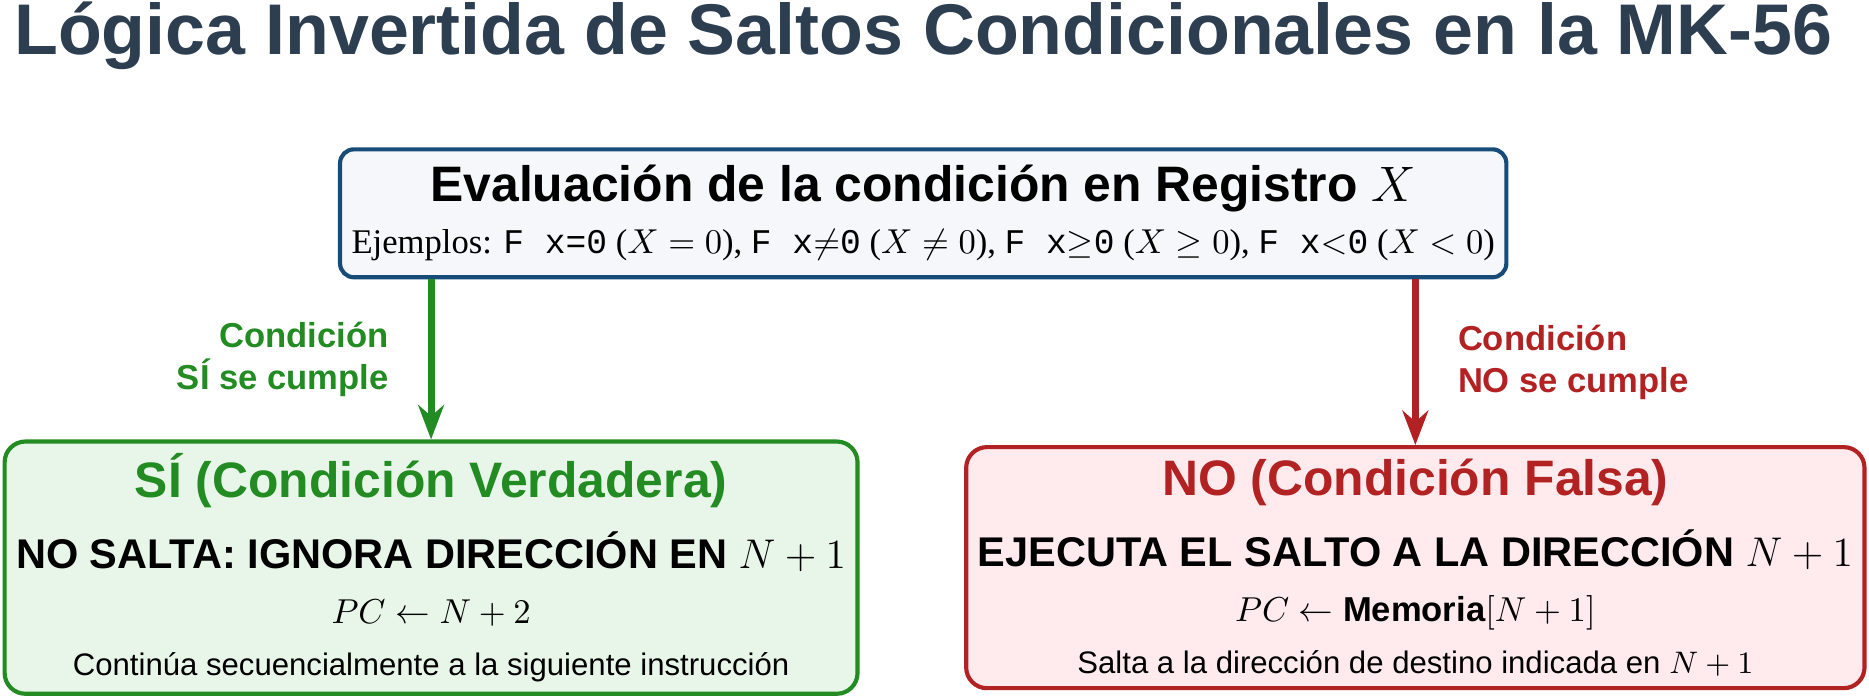
\includegraphics[width=0.95\textwidth]{figures/esquema_salto_es.png}
    \caption{Diagrama de flujo de la lógica invertida de bifurcaciones condicionales en la Elektronika MK-56.}
    \label{fig:salto_es}
\end{figure}

\subsubsection{Catálogo Formal de Condiciones Directas}
\begin{enumerate}
    \item \texttt{F x=0} (\textbf{Opcode \texttt{5E}}):
    \begin{itemize}
        \item Si $X \ne 0$ (Falso): \textbf{Salta} a la dirección de memoria en $N+1$.
        \item Si $X = 0$ (Verdadero): \textbf{No salta}; continúa la ejecución secuencial en $N+2$.
    \end{itemize}
    \item \texttt{F x$\ne$0} (\textbf{Opcode \texttt{57}}):
    \begin{itemize}
        \item Si $X = 0$ (Falso): \textbf{Salta} a la dirección de memoria en $N+1$.
        \item Si $X \ne 0$ (Verdadero): \textbf{No salta}; continúa en $N+2$.
    \end{itemize}
    \item \texttt{F x$\ge$0} (\textbf{Opcode \texttt{59}}):
    \begin{itemize}
        \item Si $X < 0$ (Falso): \textbf{Salta} a la dirección de memoria en $N+1$.
        \item Si $X \ge 0$ (Verdadero): \textbf{No salta}; continúa en $N+2$.
    \end{itemize}
    \item \texttt{F x$<$0} (\textbf{Opcode \texttt{5C}}):
    \begin{itemize}
        \item Si $X \ge 0$ (Falso): \textbf{Salta} a la dirección de memoria en $N+1$.
        \item Si $X < 0$ (Verdadero): \textbf{No salta}; continúa en $N+2$.
    \end{itemize}
\end{enumerate}

\subsubsection{Patrón Canónico de Generación de Código para Compiladores}
Para traducir una estructura condicional de alto nivel del tipo:
\begin{center}
\texttt{if (X == 0) \{ ThenBlock \} else \{ ElseBlock \}}
\end{center}
\begin{center}
\begin{tcolorbox}[colback=codebg,colframe=darkslate,width=0.95\textwidth]
\begin{verbatim}
; En paso N:
F x=0           ; Opcode 5E: Salta a else si X != 0
etiqueta_else   ; Dirección del bloque Else (paso N+1)
; Aquí inicia ThenBlock (se ejecuta si X == 0)
...
БП              ; Opcode 51: Salta incondicionalmente bloque Else
etiqueta_fin    ; Dirección de salida
etiqueta_else:
; Aquí inicia ElseBlock (alcanzado si X != 0)
...
etiqueta_fin:
\end{verbatim}
\end{tcolorbox}
\end{center}

\subsection{Contadores Automáticos de Bucle: \texttt{F L0}, \texttt{F L1}, \texttt{F L2}, \texttt{F L3}}
Instrucciones optimizadas de hardware en 2 pasos para bucles de iteración con decremento automático:
\begin{itemize}
    \item \textbf{Opcodes de Bucle:}
    \texttt{F L0} $\to$ \texttt{5Г} ($RG0$); \quad
    \texttt{F L1} $\to$ \texttt{5L} ($RG1$); \quad
    \texttt{F L2} $\to$ \texttt{58} ($RG2$); \quad
    \texttt{F L3} $\to$ \texttt{5-} ($RG3$).
    \item \textbf{Mecanismo de Ejecución:}
    \begin{enumerate}
        \item Decrementa en 1 la parte entera del registro contador:
        \[
        RGk \leftarrow RGk - 1 \qquad (k \in \{0, 1, 2, 3\})
        \]
        \item Evalúa el valor resultante en $RGk$:
        \begin{itemize}
            \item \textbf{Si $RGk \ne 0$:} El bucle prosigue; bifurca a la dirección indicada en el paso $N+1$ ($PC \leftarrow \text{Destino}$).
            \item \textbf{Si $RGk = 0$:} El bucle ha finalizado; continúa en el paso $N+2$ ($PC \leftarrow N + 2$).
        \end{itemize}
    \end{enumerate}
\end{itemize}

\begin{figure}[htbp]
    \centering
    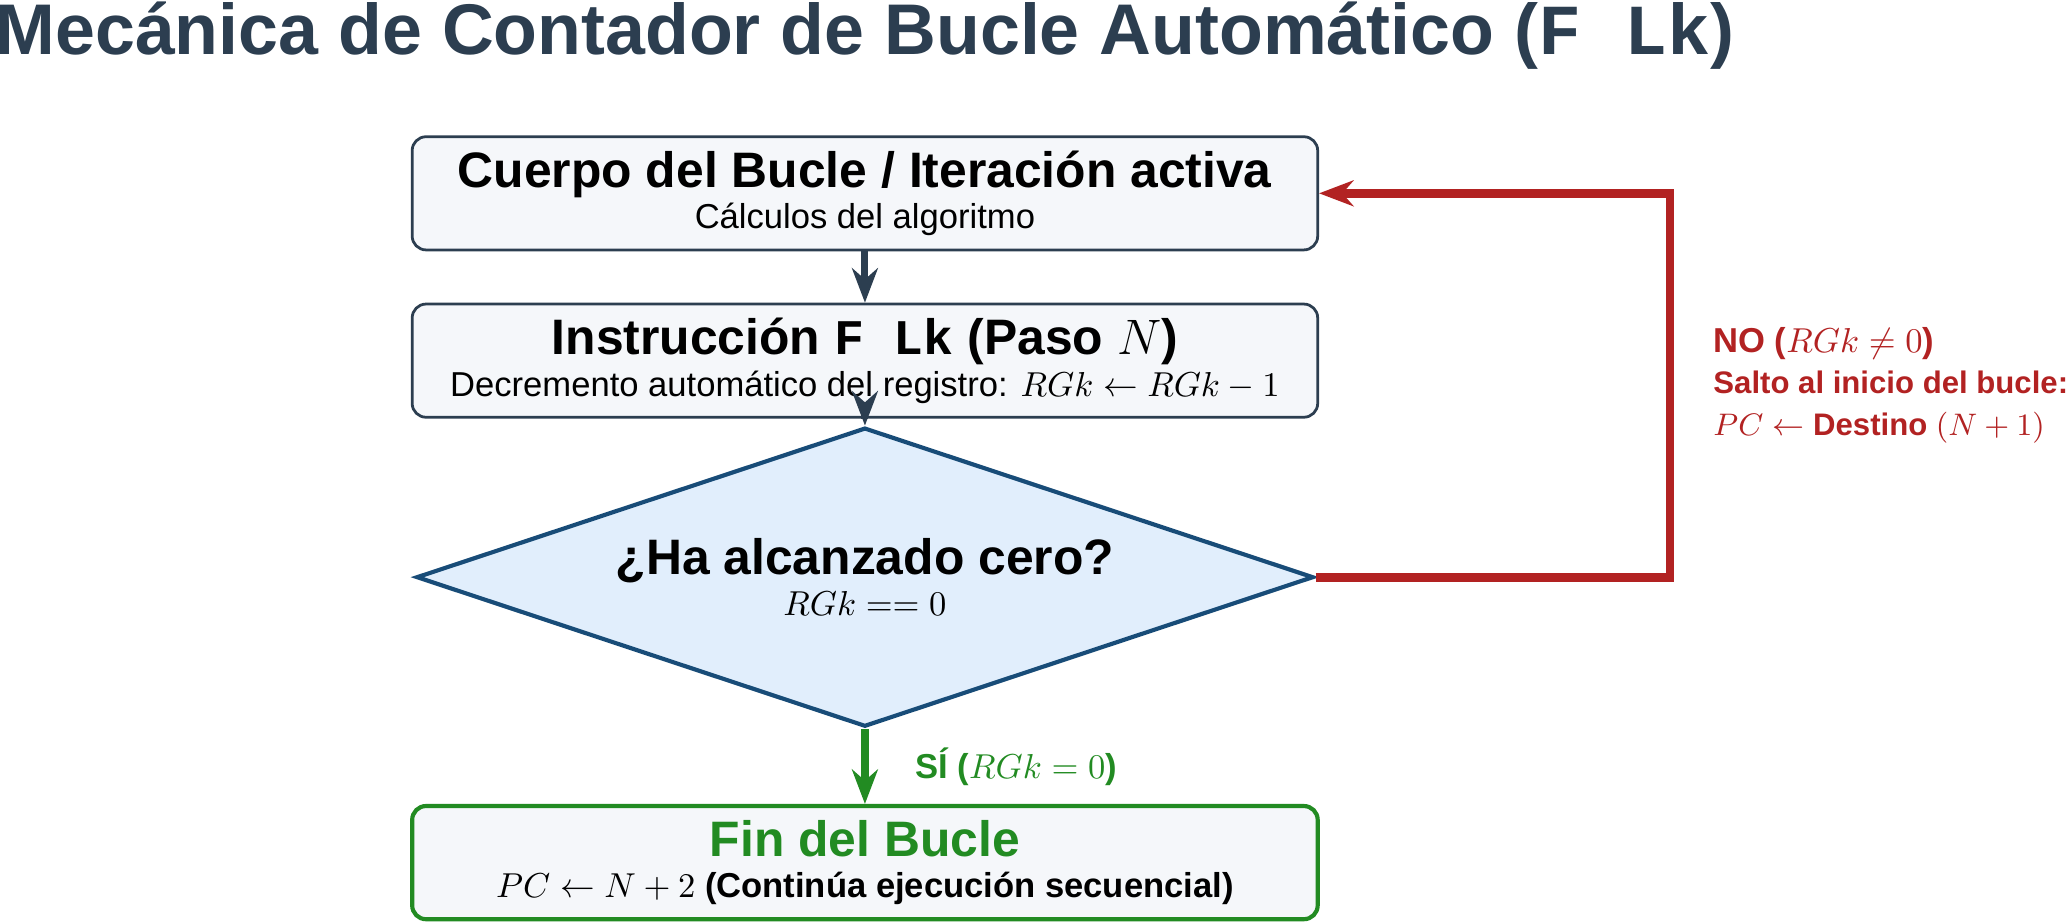
\includegraphics[width=0.88\textwidth]{figures/esquema_bucle_es.png}
    \caption{Diagrama de ciclo de control para las instrucciones de bucle por hardware (\texttt{F Lk}).}
    \label{fig:bucle_es}
\end{figure}

\subsection{Saltos Indirectos y Polimorfismo Dinámico}
La máquina permite transferencias de control donde la dirección destino se obtiene dinámicamente desde un registro de datos. Ocupan \textbf{un solo byte} en la memoria de programa:
\begin{itemize}
    \item \textbf{Salto incondicional indirecto:} \texttt{K БП [R]} (Opcodes \texttt{80} a \texttt{8Г}). Modifica $R$ (si $R \le 6$) y ramifica a la dirección contenida en $R$.
    \item \textbf{Subrutina indirecta:} \texttt{K ПП [R]} (Opcodes \texttt{-0} a \texttt{-Г}). Apila la dirección de retorno ($PC + 1$), modifica $R$ y bifurca.
    \item \textbf{Bifurcaciones condicionales indirectas:} \texttt{K x=0}, \texttt{K x$\ne$0}, \texttt{K x$\ge$0}, \texttt{K x$<$0}. Evalúan la condición en $X$; si la condición es falsa, modifican $R$ y saltan a la dirección en $R$. Si es verdadera, avanzan a $PC + 1$ sin alterar $R$.
\end{itemize}

\newpage

\section{Resumen de Especificaciones para el Desarrollador del Compilador}

\begin{center}
\renewcommand{\arraystretch}{1.2}
\setlength{\tabcolsep}{5pt}
\begin{tabular}{p{5.8cm}p{9.8cm}}
\toprule
\textbf{Parámetro de Arquitectura} & \textbf{Valor / Especificación Técnica} \\
\midrule
\textbf{Modelo de Computación} & Pila RPN (\textit{ПОЛИЗ}) pura con acumulador en la cima ($X$) \\
\textbf{Profundidad de Pila Operativa} & 4 niveles hardware: $X, Y, Z, T$ \\
\textbf{Registro de Respaldo} & 1 registro automático auxiliar: $X_1$ (\textit{Prev X}) \\
\textbf{Pila de Subrutinas} & 5 niveles LIFO independientes por hardware \\
\textbf{Capacidad de Memoria de Código} & 98 pasos direccionables (\texttt{00} a \texttt{97}) \\
\textbf{Registros de Datos} & 14 registros de coma flotante ($RG0..RG9, RGa..RGd$) \\
\textbf{Longitud de Opcodes} & 1 byte por instrucción; argumentos en el byte siguiente \\
\textbf{Semántica de Saltos Condicionales} & \textbf{Invertida:} bifurca cuando la condición es FALSA \\
\textbf{Registros con Autodecremento} & $RG0, RG1, RG2, RG3$ (resta 1 al acceder con prefijo \texttt{K}) \\
\textbf{Registros con Autoincremento} & $RG4, RG5, RG6$ (suma 1 al acceder con prefijo \texttt{K}) \\
\textbf{Contadores de Bucle por Hardware} & 4 instrucciones dedicadas: \texttt{F L0}, \texttt{F L1}, \texttt{F L2}, \texttt{F L3} \\
\textbf{Representación Hexadecimal VFD} & \texttt{0..9} estándar; \texttt{A}$\to$\texttt{-}, \texttt{B}$\to$\texttt{L}, \texttt{C}$\to$\texttt{C}, \texttt{D}$\to$\texttt{Г}, \texttt{E}$\to$\texttt{E}, \texttt{F}$\to$\textit{blanco} \\
\bottomrule
\end{tabular}
\end{center}

\subsection{Guía Práctica para la Generación de Código Intermedio (IR)}
Al implementar un generador de código desde un árbol de sintaxis abstracta (AST) o representación intermedia (IR) hacia el bytecode de la Elektronika MK-56:
\begin{enumerate}
    \item \textbf{Gestión de la Pila RPN:} El compilador debe mantener un seguimiento estático de la profundidad de la pila en tiempo de compilación. Debido a que la pila sólo cuenta con 4 niveles ($X, Y, Z, T$), expresiones complejas con más de 4 operandos concurrentes deben volcarse temporalmente a registros de datos no utilizados (por ejemplo, registros $RG7..RGd$) mediante \texttt{x$\to$П} y recuperarse posteriormente con \texttt{П$\to$x}.
    \item \textbf{Inversión de Primitivas Condicionales:} Al compilar sentencias de bifurcación condicional (\texttt{if}, \texttt{while}, \texttt{for}):
    \[
    \text{Emitir } \mathtt{F\ x=0} \implies \text{salta a la etiqueta de falla si } X \ne 0
    \]
    \[
    \text{Emitir } \mathtt{F\ x\neq0} \implies \text{salta a la etiqueta de falla si } X = 0
    \]
    \[
    \text{Emitir } \mathtt{F\ x\ge0} \implies \text{salta a la etiqueta de falla si } X < 0
    \]
    \[
    \text{Emitir } \mathtt{F\ x<0} \implies \text{salta a la etiqueta de falla si } X \ge 0
    \]
    \item \textbf{Optimización de Bucles:} Siempre que un bucle iterativo dependa de un contador entero con límite conocido en el rango $1..99$, el compilador debe asignar dicho contador a uno de los registros $RG0..RG3$ y cerrar el bucle con la instrucción \texttt{F Lk}, ahorrando así instrucciones de decremento y comparación explícitas.
\end{enumerate}

\end{document}
